\chapter{Calibration}
\label{chp:Calibration}
Data collected during the trial is used to calibrate the equations used to calculate tympanic temperature and SpO\textsubscript{2}. The calibration process for the two different vital signs are discussed separately in this chapter.

\section{Temperature Calibration}
As discussed in Section \ref{sec:Temperature related software}, the TMP006 measures die temperature, T\textsubscript{DIE}, and thermopile sensor voltage, V\textsubscript{SENSOR}. These two measurements are used to calculate the temperature of the object, T\textsubscript{OBJ}, which in the case of the Ear-Monitor is the tympanic membrane.

\medskip

Each data recording session in the trial produced 15 Ear-Monitor measurements and 3 ET 100-A benchmark measurements. Measurements from both devices are averaged separately to get one average Ear-Monitor and one average ET 100-A measurement per session. Two different calibration approaches are discussed: the group calibration approach and the intra-participant calibration approach.

\subsection{Group Calibration Approach}
In this approach, 5 recording session are used to calibrate the temperature calculation equation, Equation \ref{eq:FlatPlane}. MATLAB's curve fitting tool is used to fit a first order polynomial plane to the data points. The equation with calibration coefficients is shown by Equation \ref{eq:TempCal}.

\begin{equation}
\label{eq:TempCal}
T_{OBJ}=22.85+ 0.04803 T_{DIE}-13440 V_{SENSOR}
\end{equation}


This equation is applied to all Ear-Monitor temperature measurements. The advantage of the group calibration approach is that calibration is done only once and no patient specific calibration is needed.

\medskip

A box and whisker plot can be seen in Figure \ref{fig:BeforeAfterCalibrationBoxplot} and shows the error between the ET 100-A benchmark temperature and the Ear-Monitor temperature before and after calibration. Improvements in accuracy and precision are clearly visible in this graphical representation of the data.

\begin{figure}[H]
   \centering
   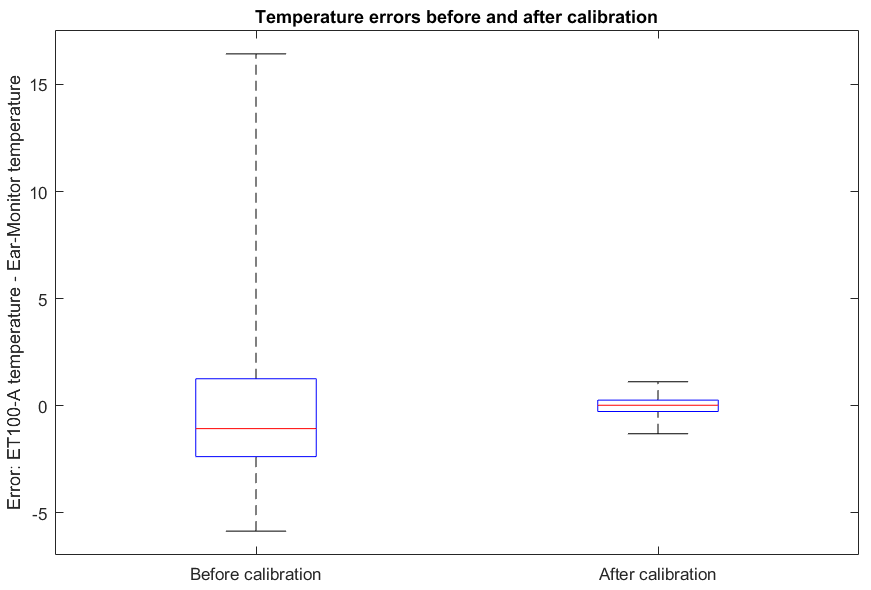
\includegraphics[width=12cm,height=7.5cm]{figs/BeforeAfterCalibrationBoxplot.png}
   \caption{Temperature errors before and after calibration}
   \label{fig:BeforeAfterCalibrationBoxplot}
\end{figure}


\subsection{Intra-participant calibration approach}
In this approach, the first recording session is used to calibrate the calibration coefficients for each participant individually. The first recording session data is entered into Equation \ref{eq:TempCal} and the error between the Ear-Monitor and ET 100-A data is used to adjust Equation \ref{eq:TempCal}.

\medskip

The advantage of this approach is that the Ear-Monitor can adjust to patient specific parameters, i.e. tympanic membrane size, the sensor's distance from the membrane and the fraction of the FOV that is occupied by the canal wall. The trade-off is that the Ear-Monitor needs to be calibrated for each participant individually. This is not a complicated process, calibration can be done in one minute and is only needed once per individual. 

\section{SpO\textsubscript{2} Calibration}
According to \cite{ti2012application} the modulated ratio, R (Equation \ref{eq:SatsRatio}), is linearly related to SpO\textsubscript{2}. The relationship they propose is given by Equation \ref{eq:SpO2_1}.

\begin{equation}
\label{eq:SpO2_1}
SpO_2=x-m\cdot R
\end{equation}

With $x$ equal to 110 and $m$ equal to 25. The relationship will vary for different pulse oximeters, and the calibration parameters for the MAX30100 in the Ear-Monitor are calculated empirically through experimentation. Equation \ref{eq:SpO2_1} is used as a starting point and the gradient, $m$, is constrained to be larger or equal to 15 in order to ensure $R$'s weight in the calculated SpO\textsubscript{2} value. The remaining calibration parameter, $x$, is systematically incremented until the desired fit is achieved. Equation \ref{eq:SpO2_2} describes the relationship between $R$ and SpO\textsubscript{2} selected for the Ear-Monitor.

\begin{equation}
\label{eq:SpO2_2}
SpO_2=106.32-15\cdot R
\end{equation}




